\documentclass[aspectratio=169]{beamer}

% Theme and appearance
\usetheme{Madrid}
\usecolortheme{default}

% Packages
\usepackage[utf8]{inputenc}
\usepackage[T1]{fontenc}
\usepackage{graphicx}
\usepackage{tikz}
\usetikzlibrary{shapes,arrows,positioning,calc,backgrounds,fit,decorations.pathmorphing}
\usepackage{array}
\usepackage{booktabs}
\usepackage{multirow}
\usepackage{colortbl}
\usepackage{xcolor}

% Graphics path for icons
\graphicspath{{images/}}

% Custom colors
\definecolor{networkblue}{RGB}{51,102,187}
\definecolor{networkgreen}{RGB}{46,125,50}
\definecolor{networkorange}{RGB}{255,152,0}
\definecolor{networkred}{RGB}{198,40,40}

% Title information
\title{Physical Infrastructure of Networks}
\author{Brendan Shea, PhD}
\institute{Rochester Community and Technical College}
\date{} % No date as requested

% Custom commands for network icons
\newcommand{\neticon}[2][0.4cm]{\includegraphics[height=#1]{#2}}

% TikZ styles for network diagrams
\tikzset{
    device/.style={rectangle, draw, thick, minimum width=2cm, minimum height=1cm, align=center},
    router/.style={rectangle, draw, thick, fill=networkblue!20, minimum width=2cm, minimum height=1cm, align=center},
    switch/.style={rectangle, draw, thick, fill=networkgreen!20, minimum width=2cm, minimum height=1cm, align=center},
    computer/.style={rectangle, draw, thick, fill=gray!20, minimum width=1.5cm, minimum height=1cm, align=center},
    connection/.style={thick, -latex},
    wireless/.style={thick, -latex, dashed, color=networkblue},
    cloud/.style={ellipse, draw, thick, fill=networkorange!10, minimum width=3cm, minimum height=2cm, align=center}
}

\begin{document}

\begin{frame}
    \titlepage
\end{frame}

% Slide 1: Module Introduction
\begin{frame}{The Physical Network: Why Cables Still Matter}
            
            \begin{itemize}
                \item Every like, text, and video depends on physical cables carrying electrical or light signals.
                \item Understanding the physical layer helps you troubleshoot problems and design reliable networks.
                \item We'll explore copper cables, fiber optics, and how to install them properly.
                \item By the end, you'll know how to choose the right cable for any networking situation.
            \end{itemize}
       
            \begin{tikzpicture}[scale=1.2, every node/.style={scale=1.2}]
                % Phone
                \node at (0,3) {\neticon[0.6cm]{icon_phone.png}};
                \node[below, font=\tiny] at (0,2.7) {Your Phone};
                
                % Router
                \node at (2,3) {\neticon[0.6cm]{icon_router.png}};
                \node[below, font=\tiny] at (2,2.7) {Home Router};
                
                % Internet
                \node at (4,3) {\neticon[0.7cm]{icon_internet.png}};
                \node[below, font=\tiny] at (4,2.6) {Internet};
                
                % Server
                \node at (6,3) {\neticon[0.6cm]{icon_server.png}};
                \node[below, font=\tiny] at (6,2.7) {Netflix Server};
                
                % Connections with cable labels
                \draw[->, thick, networkblue] (0.3,3) -- (1.7,3);
                \node[above, font=\tiny, networkblue] at (1,3) {WiFi};
                
                \draw[->, thick, networkgreen] (2.3,3) -- (3.7,3);
                \node[above, font=\tiny, networkgreen] at (3,3) {Cable};
                
                \draw[->, thick, networkorange] (4.3,3) -- (5.7,3);
                \node[above, font=\tiny, networkorange] at (5,3) {Fiber};
                
                % Data representation
                \node[font=\tiny, text width=2cm, align=center] at (3,1.5) {All transmitted as electrical or light signals through physical cables!};
            \end{tikzpicture}
\end{frame}

% Slide 2: How Networks Transmit Data
\begin{frame}{How Networks Transmit Data}
    \begin{itemize}
        \item Networks transmit data as \textbf{digital signals}, which are patterns of electrical voltages or light pulses representing 1s and 0s.
        \item Think of it like Morse code: just as dots and dashes can spell words, 1s and 0s can represent any information.
        \item A \textbf{bit} is a single binary digit (1 or 0), and 8 bits make a \textbf{byte} (enough to represent one letter).
        \item \textbf{Bandwidth} measures how many bits can be transmitted per second, like the width of a pipe determining water flow.
    \end{itemize}
    
    \vspace{0.5cm}
    \begin{block}{Key Insight}
        Your computer turns everything---text, images, videos---into billions of 1s and 0s, then cables carry these as electrical or light signals at incredible speeds.
    \end{block}
\end{frame}

% Slide 3: Introduction to Ethernet
\begin{frame}{Introduction to Ethernet}
    \begin{itemize}
        \item \textbf{Ethernet} is the standard set of rules (protocols) that computers use to communicate over wired networks.
        \item Invented in the 1970s at Xerox, Ethernet has evolved from thick coaxial cables to today's twisted pair cables.
        \item Ethernet became the dominant standard because it's reliable, affordable, and continuously improves without requiring complete replacement.
        \item When you plug a cable into your computer or router, you're almost certainly using Ethernet technology.
    \end{itemize}
    
    \vspace{0.5cm}
    \begin{alertblock}{Why It Matters}
        Over 90\% of wired networks worldwide use Ethernet standards, making it essential knowledge for any network technician.
    \end{alertblock}
\end{frame}

% Slide 4: Copper Cables Overview
\begin{frame}{Copper Cables Overview}
    \begin{columns}[T]
        \begin{column}{0.55\textwidth}
            \begin{itemize}
                \item \textbf{Copper cables} use copper wire to conduct electrical signals because copper is highly conductive, flexible, and cost-effective.
                \item The two main types are \textbf{twisted pair} (multiple wires twisted together) and \textbf{coaxial} (center wire surrounded by insulation and shield).
                \item Twisted pair cables connect most computers, phones, and network devices in homes, schools, and offices.
                \item Coaxial cables are commonly used for cable TV and internet connections from your Internet Service Provider.
            \end{itemize}
        \end{column}
        \begin{column}{0.4\textwidth}
            \centering
            \includegraphics[width=0.9\textwidth]{UTP_cable_w_twists_showing.jpg}
            \vspace{0.2cm}
            
            \small{\textit{Twisted pair cable showing the twisted wire pairs inside}}
        \end{column}
    \end{columns}
\end{frame}

% Slide 5: Unshielded Twisted Pair (UTP) Cable
\begin{frame}{Unshielded Twisted Pair (UTP) Cable}
    \begin{columns}[T]
        \begin{column}{0.55\textwidth}
            \begin{itemize}
                \item \textbf{Unshielded Twisted Pair (UTP)} is the most common type of network cable, found in homes, schools, and most businesses.
                \item UTP contains 8 copper wires arranged in 4 color-coded pairs, with each pair twisted together at specific rates.
                \item The twisting reduces \textbf{electromagnetic interference (EMI)} by canceling out electrical noise that could corrupt the signal.
                \item UTP is "unshielded" because it has no metal foil or braiding protecting the wires---it relies entirely on twisting for protection.
            \end{itemize}
        \end{column}
        \begin{column}{0.4\textwidth}
            \centering
            \includegraphics[width=0.95\textwidth]{UTP-cable-cross-section.png}
            \vspace{0.2cm}
            
            \small{\textit{Cross-section showing 4 twisted pairs inside the cable jacket}}
        \end{column}
    \end{columns}
\end{frame}

% Slide 6: Shielded Cables (STP/ScTP)
\begin{frame}{Shielded and Screened Twisted Pair Cables}
    \begin{columns}[T]
        \begin{column}{0.55\textwidth}
            \begin{itemize}
                \item \textbf{Shielded Twisted Pair (STP)} cables have metal foil or braided shielding around the wire pairs to provide extra protection from interference.
                \item These cables are necessary in environments with high electromagnetic interference, such as near motors, fluorescent lights, or heavy machinery.
                \item The trade-offs include higher cost (30-50\% more expensive), reduced flexibility, and more difficult installation.
                \item \textbf{Screened Twisted Pair (ScTP)} uses an overall shield around all pairs, while STP may shield individual pairs as well.
            \end{itemize}
        \end{column}
        \begin{column}{0.4\textwidth}
            \centering
            \includegraphics[width=0.85\textwidth]{S-FTP_CAT_7.jpg}
            \vspace{0.2cm}
            
            \small{\textit{Shielded Cat 7 cable showing individual pair shielding and overall shield}}
        \end{column}
    \end{columns}
\end{frame}

% Slide 7: Cable Categories (Cat Standards)
\begin{frame}{Cable Categories (Cat Standards)}
    \begin{itemize}
        \item The \textbf{Category (Cat)} rating system classifies twisted pair cables by their performance specifications---higher numbers mean better performance.
        \item Each category specifies maximum bandwidth, supported speeds, and maximum cable length (usually 100 meters).
        \item Choosing the right category depends on your current needs and future upgrade plans.
    \end{itemize}
    
    \vspace{0.3cm}
    \begin{table}
        \centering
        \small
        \begin{tabular}{|l|c|c|l|}
            \hline
            \rowcolor{networkblue!20}
            \textbf{Category} & \textbf{Max Speed} & \textbf{Bandwidth} & \textbf{Common Use} \\
            \hline
            Cat 5e & 1 Gbps & 100 MHz & Standard for homes/offices \\
            \hline
            Cat 6 & 1-10 Gbps & 250 MHz & Business networks \\
            \hline
            Cat 6a & 10 Gbps & 500 MHz & High-performance networks \\
            \hline
            Cat 7 & 10 Gbps & 600 MHz & Data centers (shielded) \\
            \hline
            Cat 8 & 25-40 Gbps & 2000 MHz & Server connections \\
            \hline
        \end{tabular}
    \end{table}
    
    \vspace{0.2cm}
    \small{\textit{Note: All support 100 meter maximum distance for full specifications}}
\end{frame}

% Slide 8: RJ-45 Connectors
\begin{frame}{RJ-45 Connectors}
    \begin{columns}[T]
        \begin{column}{0.55\textwidth}
            \begin{itemize}
                \item The \textbf{RJ-45 connector} is the standard plastic connector with 8 pins that plugs into network devices.
                \item Each of the 8 pins corresponds to one of the 8 wires inside the twisted pair cable.
                \item Connectors can be \textbf{crimped} directly onto cable ends (requires special tool) or cables can terminate at \textbf{keystone jacks} in wall plates.
                \item The clear plastic housing lets you visually inspect the wire connections to verify correct installation.
            \end{itemize}
        \end{column}
        \begin{column}{0.4\textwidth}
            \centering
            \includegraphics[width=0.85\textwidth]{RJ45s.jpg}
            \vspace{0.2cm}
            
            \small{\textit{RJ-45 connectors showing the 8 pins and wire arrangement}}
            
            \vspace{0.3cm}
            \includegraphics[width=0.9\textwidth]{RJ45_connect.png}
        \end{column}
    \end{columns}
\end{frame}

% Slide 9: Ethernet Speed Standards
\begin{frame}{Ethernet Speed Standards}
    \begin{itemize}
        \item Ethernet standards use a naming convention: \textbf{speed-transmission type-media type} (e.g., 1000BASE-T means 1000 Mbps, baseband, twisted pair).
        \item \textbf{10BASE-T} (10 Mbps) was the original standard, now obsolete but important historically.
        \item \textbf{100BASE-TX} (Fast Ethernet) runs at 100 Mbps and uses only 2 of the 4 wire pairs in Cat 5e or better cable.
        \item \textbf{1000BASE-T} (Gigabit Ethernet) runs at 1000 Mbps (1 Gbps), uses all 4 wire pairs, and requires Cat 5e minimum with Cat 6 recommended.
    \end{itemize}
    
    \vspace{0.3cm}
    \begin{table}
        \centering
        \small
        \begin{tabular}{|l|c|c|c|}
            \hline
            \rowcolor{networkgreen!20}
            \textbf{Standard} & \textbf{Speed} & \textbf{Wire Pairs} & \textbf{Min. Cable} \\
            \hline
            100BASE-TX & 100 Mbps & 2 pairs & Cat 5e \\
            \hline
            1000BASE-T & 1 Gbps & 4 pairs & Cat 5e \\
            \hline
            10GBASE-T & 10 Gbps & 4 pairs & Cat 6a \\
            \hline
        \end{tabular}
    \end{table}
\end{frame}

% Slide 10: Coaxial and Twinaxial Cables
\begin{frame}{Coaxial and Twinaxial Cable}
    \begin{columns}[T]
        \begin{column}{0.55\textwidth}
            \begin{itemize}
                \item \textbf{Coaxial cable} has a completely different design: a single center conductor surrounded by insulation, a braided shield, and an outer jacket.
                \item The shield protects the center conductor from interference and prevents signal leakage, making coax more resistant to EMI than unshielded twisted pair.
                \item Common connectors include \textbf{F-type} (cable TV/internet) and \textbf{BNC} (older networks and video equipment).
                \item \textbf{Twinaxial cable} (twinax) uses two inner conductors and is used for short, high-speed data center connections.
            \end{itemize}
        \end{column}
        \begin{column}{0.4\textwidth}
            \centering
            \includegraphics[width=0.95\textwidth]{Coaxial_cable_cutaway.png}
            \vspace{0.3cm}
            
            \includegraphics[width=0.6\textwidth]{F_connector_male.jpg}
            
            \small{\textit{Coaxial cable construction and F-type connector}}
        \end{column}
    \end{columns}
\end{frame}

% Slide 11: CASE STUDY - Problem
\begin{frame}{Case Study: The Addams Family Network}
    \begin{block}{The Scenario}
        Wednesday Addams is rewiring the mansion's network. She needs to connect 4 computers in the torture chamber (basement) to the family router located in Gomez's office on the second floor---a distance of 150 feet through the mansion's walls.
        
        \vspace{0.3cm}
        The basement has significant electrical interference from Fester's experimental equipment, which frequently generates electromagnetic pulses. The family wants fast, reliable connections for streaming horror movies and conducting paranormal research.
    \end{block}
    
    \vspace{0.5cm}
    \textbf{Your Task:}
    \begin{itemize}
        \item What type and category of cable should Wednesday use?
        \item Justify your choice considering distance, interference, speed, and cost.
        \item Are there any alternatives she should consider?
    \end{itemize}
\end{frame}

% Slide 12: CASE STUDY - Solution
\begin{frame}{Case Study: Solution}
    \textbf{Recommended Solution:} Cat 6 or Cat 6a STP (Shielded Twisted Pair)
    
    \vspace{0.3cm}
    \begin{itemize}
        \item \textbf{Distance Check:} 150 feet = 45.7 meters, well under the 100-meter (328 feet) limit for Ethernet {\color{networkgreen}\checkmark}
        \item \textbf{Speed:} Cat 6 supports 1 Gbps (sufficient for streaming), Cat 6a supports 10 Gbps (future-proof) {\color{networkgreen}\checkmark}
        \item \textbf{Interference:} Uncle Fester's equipment requires shielded cable; regular UTP would experience frequent dropouts {\color{networkgreen}\checkmark}
        \item \textbf{Cost Analysis:} STP costs 30-50\% more than UTP, but necessary for reliability in high-EMI environment
    \end{itemize}
    
    \vspace{0.3cm}
    \begin{alertblock}{Alternative Option}
        If the interference proves too severe even for STP, Wednesday might consider fiber optic cable, which is completely immune to electromagnetic interference---though it's more expensive and harder to terminate.
    \end{alertblock}
\end{frame}

% Slide 13: Understanding MAC Addresses and Collision Domains
\begin{frame}{MAC Addresses and Collision Domains}
    \begin{itemize}
        \item Every network device has a unique \textbf{Media Access Control (MAC) address}, a 48-bit identifier burned into the network interface card at manufacturing.
        \item Think of a MAC address as your device's permanent physical "home address"---it never changes (e.g., 00:1A:2B:3C:4D:5E).
        \item A \textbf{collision domain} is a network segment where data packets can collide if two devices transmit simultaneously.
        \item Modern \textbf{switches} create separate collision domains for each port, preventing collisions and improving network performance dramatically compared to old hubs.
    \end{itemize}
    
    \vspace{0.3cm}
    \begin{block}{Why This Matters}
        Understanding collision domains explains why switches are superior to hubs---each device gets dedicated bandwidth instead of sharing and competing for access.
    \end{block}
\end{frame}

% Slide 14: 100BASE-TX Fast Ethernet
\begin{frame}{100BASE-TX Fast Ethernet}
    \begin{itemize}
        \item \textbf{100BASE-TX} (Fast Ethernet) operates at 100 Megabits per second, which is 10 times faster than the original 10BASE-T standard.
        \item This standard only uses 2 of the 4 wire pairs in the cable: one pair for transmitting and one pair for receiving data.
        \item Fast Ethernet requires Cat 5e or better cable and can reach distances up to 100 meters (328 feet).
        \item While Gigabit Ethernet is now more common, you'll still find 100BASE-TX in older networks and devices like IP cameras or printers.
    \end{itemize}
    
    \vspace{0.3cm}
    \begin{alertblock}{Legacy Technology}
        Many organizations still have 100BASE-TX equipment in use---knowing how to work with it is essential for technicians supporting existing infrastructure.
    \end{alertblock}
\end{frame}

% Slide 15: Gigabit Ethernet (1000BASE-T)
\begin{frame}{Gigabit Ethernet (1000BASE-T)}
    \begin{itemize}
        \item \textbf{1000BASE-T} (Gigabit Ethernet) transmits data at 1000 Megabits per second (1 Gbps), providing 10 times the speed of Fast Ethernet.
        \item Unlike Fast Ethernet, Gigabit uses all 4 wire pairs simultaneously, with each pair both transmitting and receiving at the same time.
        \item This standard requires Cat 5e cable at minimum, though Cat 6 is strongly recommended for reliability and future-proofing.
        \item Gigabit Ethernet is currently the standard for most home and business networks, offering excellent performance at reasonable cost.
    \end{itemize}
    
    \vspace{0.3cm}
    \begin{block}{Design Choice}
        When installing new networks today, always use Cat 6 or better cable even if current devices only need Fast Ethernet---this prepares for inevitable upgrades.
    \end{block}
\end{frame}

% Slide 16: Higher-Speed Ethernet Standards
\begin{frame}{Higher-Speed Ethernet Standards}
    \begin{itemize}
        \item \textbf{10GBASE-T} (10 Gigabit Ethernet) operates at 10,000 Mbps and requires Cat 6a cable or better to reach the full 100-meter distance.
        \item \textbf{25GBASE-T} and \textbf{40GBASE-T} are emerging standards primarily used for server-to-switch connections in data centers.
        \item These ultra-high-speed standards use more sophisticated encoding and require higher-quality cables to combat signal degradation.
        \item Most homes and small businesses don't need speeds beyond 1 Gbps currently, but large organizations use 10+ Gbps for backbone connections and server farms.
    \end{itemize}
    
    \vspace{0.3cm}
    \begin{table}
        \centering
        \small
        \begin{tabular}{|l|c|c|}
            \hline
            \rowcolor{networkorange!20}
            \textbf{Standard} & \textbf{Speed} & \textbf{Typical Use} \\
            \hline
            1000BASE-T & 1 Gbps & Workstations, most networks \\
            \hline
            10GBASE-T & 10 Gbps & Servers, backbone links \\
            \hline
            25/40GBASE-T & 25-40 Gbps & Data center core \\
            \hline
        \end{tabular}
    \end{table}
\end{frame}

% Slide 17: Introduction to Structured Cabling Systems
\begin{frame}{Introduction to Structured Cabling Systems}
    \begin{itemize}
        \item A \textbf{structured cabling system} is an organized, standardized approach to network cabling that provides a "blueprint" for how cables should be installed throughout a building.
        \item Without structure, cable installations become "spaghetti"---tangled, impossible to trace, and nearly impossible to troubleshoot or modify.
        \item The system divides the network into hierarchical subsystems: work areas (where users work), horizontal cabling (floor distribution), and backbone cabling (between floors/buildings).
        \item Following structured cabling standards ensures that any qualified technician can understand and work with your installation, even years later.
        \item Properly designed structured cabling can last 15-20 years, supporting multiple technology upgrades without rewiring.
    \end{itemize}
\end{frame}

% Slide 18: Structured Cabling Components
\begin{frame}{Structured Cabling Components}
    \begin{columns}[T]
        \begin{column}{0.5\textwidth}
            \begin{itemize}
                \item \textbf{Work Area Outlet}: Wall jack where users plug in devices (maximum 3 meters of patch cable to device).
                \item \textbf{Horizontal Cabling}: Permanent cable running from work area to telecommunications room (maximum 90 meters).
                \item \textbf{Telecommunications Room (TR)}: Central wiring closet on each floor with patch panels and switches.
                \item \textbf{Backbone Cabling}: Connects TRs across floors or between buildings.
            \end{itemize}
        \end{column}
        \begin{column}{0.45\textwidth}
            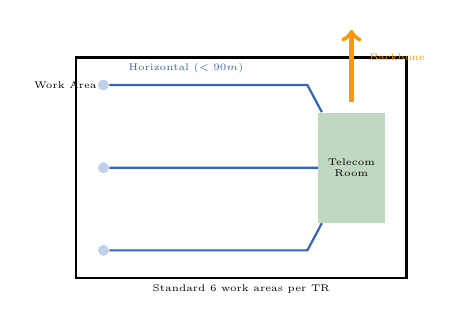
\begin{tikzpicture}[scale=0.7, every node/.style={transform shape}]
                % Floor layout
                \draw[thick] (0,0) rectangle (6,4);
                
                % Work area outlets
                \node[fill=networkblue!30, circle, inner sep=2pt] (wa1) at (0.5,3.5) {};
                \node[fill=networkblue!30, circle, inner sep=2pt] (wa2) at (0.5,2) {};
                \node[fill=networkblue!30, circle, inner sep=2pt] (wa3) at (0.5,0.5) {};
                \node[font=\tiny, left] at (wa1) {Work Area};
                
                % TR
                \node[fill=networkgreen!30, rectangle, minimum width=1.2cm, minimum height=2cm] (tr) at (5,2) {};
                \node[font=\tiny, text width=1cm, align=center] at (tr) {Telecom Room};
                
                % Horizontal runs
                \draw[networkblue, thick] (wa1) -- (4.2,3.5) -- (tr);
                \draw[networkblue, thick] (wa2) -- (tr);
                \draw[networkblue, thick] (wa3) -- (4.2,0.5) -- (tr);
                
                % Backbone (going up)
                \draw[networkorange, ultra thick, ->] (5,3.2) -- (5,4.5);
                \node[font=\tiny, right, networkorange] at (5.2,4) {Backbone};
                
                % Labels
                \node[font=\tiny, networkblue] at (2,3.8) {Horizontal ($< 90m$)};
                
                % Legend
                \node[font=\tiny, below] at (3,0) {Standard 6 work areas per TR};
            \end{tikzpicture}
        \end{column}
    \end{columns}
\end{frame}

% Slide 19: T568A and T568B Termination Standards
\begin{frame}{T568A and T568B Wiring Standards}
    \begin{columns}[T]
        \begin{column}{0.5\textwidth}
            \begin{itemize}
                \item \textbf{T568A} and \textbf{T568B} are two different standards for arranging the 8 wires within an RJ-45 connector.
                \item The standards differ only in the positions of the orange and green pairs---all other wires are identical.
                \item A \textbf{straight-through cable} uses the same standard on both ends (most common), while a \textbf{crossover cable} uses different standards on each end.
                \item Consistency matters more than which standard you choose---pick one and use it throughout your entire installation.
            \end{itemize}
        \end{column}
        \begin{column}{0.45\textwidth}
            \centering
            \includegraphics[width=0.85\textwidth]{T568A_pins.png}
            
            \vspace{0.3cm}
            \includegraphics[width=0.85\textwidth]{T565B_pins.png}
            
            \vspace{0.2cm}
            \small{\textit{T568A (top) and T568B (bottom) pin assignments}}
        \end{column}
    \end{columns}
\end{frame}

% Slide 20: Patch Panels - The Organized Network
\begin{frame}{Patch Panels: The Organized Network}
    \begin{columns}[T]
        \begin{column}{0.5\textwidth}
            \begin{itemize}
                \item A \textbf{patch panel} serves as the central connection point in a telecommunications room where all horizontal cables terminate.
                \item The front of the panel has RJ-45 ports labeled for each cable run; the back has punch-down blocks where wires are terminated.
                \item Patch panels make troubleshooting easier by providing a single, organized location to test and reroute connections without touching permanent wiring.
                \item Short \textbf{patch cables} connect from the patch panel to switches, allowing flexible network configuration changes.
            \end{itemize}
        \end{column}
        \begin{column}{0.45\textwidth}
            \centering
            \includegraphics[width=0.95\textwidth]{patch_panel.png}
            
            \vspace{0.3cm}
            \small{\textit{24-port patch panel with labeled ports}}
            
            \vspace{0.2cm}
            \begin{alertblock}{Pro Tip}
                Always label both ends of every cable and document which patch panel port goes to which room!
            \end{alertblock}
        \end{column}
    \end{columns}
\end{frame}

% Slide 21: Cable Installation Best Practices
\begin{frame}{Cable Installation Best Practices}
    \begin{itemize}
        \item \textbf{Plenum-rated cables} (CMP) must be used in air handling spaces because they produce less toxic smoke in fires; \textbf{riser-rated cables} (CMR) are for vertical shafts between floors.
        \item Never exceed the cable's \textbf{minimum bend radius} (typically 4 times the cable diameter)---sharp bends damage internal wires and degrade performance.
        \item Maintain proper cable management with no kinks, avoid running parallel to electrical cables (maintain 12+ inches separation), and never exceed maximum pulling tension (25 lbs for Cat 6).
        \item Label everything immediately during installation: both cable ends, patch panel ports, wall jacks, and create detailed documentation showing cable routes.
    \end{itemize}
    
    \vspace{0.3cm}
    \begin{alertblock}{Critical Safety Rule}
        Building codes legally require specific cable ratings for different locations---using the wrong cable type can result in failed inspections, fines, and serious fire hazards.
    \end{alertblock}
\end{frame}

% Slide 22: Tools of the Trade
\begin{frame}{Cable Installation Tools}
    \begin{columns}[T]
        \begin{column}{0.55\textwidth}
            \begin{itemize}
                \item \textbf{Punch-down tools} (with 110 blade) are used to terminate wires onto patch panels and keystone jacks by forcing the wire into the connector and cutting off excess.
                \item \textbf{Cable strippers} remove the outer jacket without damaging internal wires, while \textbf{crimpers} attach RJ-45 connectors to cable ends.
                \item \textbf{Cable testers} verify that all 8 wires are correctly connected and detect opens, shorts, and miswires.
                \item \textbf{Tone generators} send a signal through a cable while a probe traces the cable to identify which physical cable corresponds to which connection.
            \end{itemize}
        \end{column}
        \begin{column}{0.4\textwidth}
            \centering
            \includegraphics[width=0.45\textwidth]{punch_down.png}
            
            \vspace{0.2cm}
            \includegraphics[width=0.45\textwidth]{cable_crimper.png}
            
            \vspace{0.2cm}
            \includegraphics[width=0.45\textwidth]{cable_tester.png}
        \end{column}
    \end{columns}
\end{frame}

% Slide 23: CASE STUDY - Problem
\begin{frame}{Case Study: The Addams Family Crypt Network}
    \begin{block}{The Scenario}
        \scriptsize
        Morticia wants to add network connectivity to the family crypt in the basement for livestreaming séances. The router is in Gomez's office on the second floor. The cable must run 65 meters through the mansion's ceiling plenum (the old ventilation system), then 20 meters down a vertical shaft behind the walls to reach the crypt.
        
        \vspace{0.3cm}
        Thing has found three boxes of cable in the attic:
        \begin{itemize}
            \item Cat 6 standard PVC jacket (CMG rated)
            \item Cat 6 Plenum rated (CMP) 
            \item Cat 6 Riser rated (CMR)
        \end{itemize}
    \end{block}
    
    \vspace{0.3cm}
    \textbf{Your Task:}
    \begin{itemize}
        \item Which cable(s) should Morticia use for each part of the run?
        \item Will the total distance work for Gigabit Ethernet?
        \item What happens if she uses the wrong cable type?
    \end{itemize}
\end{frame}

% Slide 24: CASE STUDY - Solution
\begin{frame}{Case Study: Solution}
    \textbf{Best Solution:} Cat 6 Plenum-rated (CMP) cable for the entire run
    
    \textbf{Alternative:} CMP for plenum section (65m) + CMR for riser section (20m)
    
    \vspace{0.3cm}
    \begin{itemize}
        \item \textbf{Distance Check:} 85 meters total is under the 90-meter horizontal limit (100m with patch cables) {\color{networkgreen}\checkmark}
        \item \textbf{Plenum Section:} MUST use CMP-rated cable---CMR or CMG would violate fire codes {\color{networkred}X}
        \item \textbf{Riser Section:} Could use CMR or CMP (CMP works everywhere, CMR only in vertical shafts)
        \item \textbf{Practical Choice:} Using CMP throughout is simpler and ensures compliance everywhere
    \end{itemize}
    
    \vspace{0.3cm}
    \begin{alertblock}{What Goes Wrong?}
        Using CMG anywhere: Fails building inspection, expensive rewiring. Using CMR in the plenum: Fire hazard---toxic fumes could spread through ventilation. The mansion's insurance company would not be pleased!
    \end{alertblock}
\end{frame}

% Slide 25: Why Fiber Optic Cables?
\begin{frame}{Why Fiber Optic Cables?}
    \begin{itemize}
        \item Copper cables have fundamental limitations: maximum distance of 100 meters, susceptibility to electromagnetic interference, and speed limits around 10 Gbps for twisted pair.
        \item \textbf{Fiber optic cables} use pulses of light instead of electrical signals, completely eliminating electromagnetic interference problems.
        \item Fiber provides dramatically longer distances (up to 40+ kilometers for single-mode), much higher speeds (100+ Gbps), and improved security (difficult to tap).
        \item The trade-offs include higher initial cost, more fragile physical properties, and requirement for specialized tools and training for installation.
    \end{itemize}
    
    \vspace{0.3cm}
    \begin{block}{When to Choose Fiber}
        Use fiber for: connections between buildings, long runs within buildings (>100m), environments with heavy EMI, high-security applications, and backbone connections requiring 10+ Gbps speeds.
    \end{block}
\end{frame}

% Slide 26: How Fiber Optic Cables Work
\begin{frame}{How Fiber Optic Cables Work}
    \begin{columns}[T]
        \begin{column}{0.5\textwidth}
            \begin{itemize}
                \item Light pulses represent digital data: light on = 1, light off = 0, transmitted billions of times per second.
                \item The light travels through a glass or plastic core using \textbf{total internal reflection}---light bounces off the walls at specific angles, staying contained within the fiber.
                \item Think of it like a slide at a water park: the walls keep water from spilling out as it travels down, just as the cladding keeps light inside the core.
                \item Light sources can be LEDs (cheaper, shorter distance) or lasers (expensive, longer distance, more precise).
            \end{itemize}
        \end{column}
        \begin{column}{0.45\textwidth}
            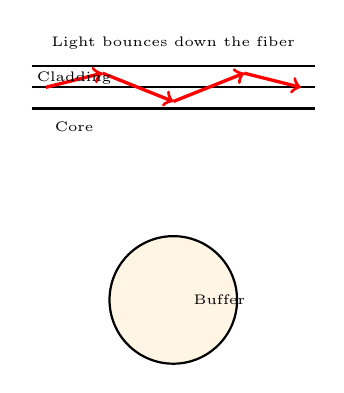
\begin{tikzpicture}[scale=0.9]
                % Fiber optic cable cross-section
                \draw[thick, fill=networkblue!30] (0,0) circle (0.3cm);
                \node[font=\tiny] at (0,0) {Core};
                
                \draw[thick, fill=networkgreen!20] (0,0) circle (0.6cm);
                \node[font=\tiny] at (0,-0.45) {Cladding};
                
                \draw[thick, fill=networkorange!10] (0,0) circle (0.9cm);
                \node[font=\tiny] at (0.65,0) {Buffer};
                
                % Light ray showing reflection
                \begin{scope}[yshift=3cm]
                    \draw[thick] (-2,0) -- (2,0);
                    \draw[thick] (-2,0.3) -- (2,0.3);
                    \draw[thick] (-2,-0.3) -- (2,-0.3);
                    
                    % Light ray
                    \draw[->, red, very thick] (-1.8,0) -- (-1,0.2);
                    \draw[->, red, very thick] (-1,0.2) -- (0,-0.2);
                    \draw[->, red, very thick] (0,-0.2) -- (1,0.2);
                    \draw[->, red, very thick] (1,0.2) -- (1.8,0);
                    
                    \node[font=\tiny, above] at (0,0.4) {Light bounces down the fiber};
                    \node[font=\tiny, below] at (-1.4,-0.35) {Core};
                    \node[font=\tiny, below] at (-1.4,0.35) {Cladding};
                \end{scope}
            \end{tikzpicture}
        \end{column}
    \end{columns}
\end{frame}

% Slide 27: Fiber Cable Construction
\begin{frame}{Fiber Cable Construction}
    \begin{columns}[T]
        \begin{column}{0.55\textwidth}
            \begin{itemize}
                \item The \textbf{core} is the ultra-thin glass center where light actually travels---only 9 to 62.5 micrometers ($\mu$m) in diameter (thinner than a human hair).
                \item The \textbf{cladding} surrounds the core with a different glass that has a lower refractive index, causing light to reflect back into the core.
                \item A \textbf{buffer coating} protects the fragile glass from moisture and physical damage.
                \item \textbf{Strengthening fibers} (often Kevlar) provide tensile strength, and the \textbf{outer jacket} protects everything.
            \end{itemize}
        \end{column}
        \begin{column}{0.4\textwidth}
            \centering
            \includegraphics[width=0.95\textwidth]{Multi_fiber_cable_cutaway.jpg}
            
            \vspace{0.3cm}
            \small{\textit{Multi-fiber cable showing individual fibers, strengthening materials, and jacket}}
            
            \vspace{0.2cm}
            \begin{alertblock}{Handle with Care!}
                Fiber is glass---it can break if bent too sharply or pulled too hard!
            \end{alertblock}
        \end{column}
    \end{columns}
\end{frame}

% Slide 28: Single-Mode vs. Multimode Fiber
\begin{frame}{Single-Mode vs. Multimode Fiber}
    \begin{itemize}
        \item \textbf{Single-mode fiber (SMF)} has a tiny 9-micrometer ($\mu$m) core that allows only one light path, using laser light sources for precise transmission.
        \item \textbf{Multimode fiber (MMF)} has a larger 50 or 62.5-micrometer ($\mu$m) core allowing multiple light paths, using cheaper LED light sources.
        \item Single-mode supports much longer distances (40+ km) but costs more for equipment; multimode is cheaper but limited to shorter distances (typically 550 meters or less).
    \end{itemize}
    
    \vspace{0.3cm}
    \begin{table}
        \centering
        \small
        \begin{tabular}{|l|c|c|}
            \hline
            \rowcolor{networkblue!20}
            \textbf{Feature} & \textbf{Single-Mode (SMF)} & \textbf{Multimode (MMF)} \\
            \hline
            Core Diameter & 9 $\mu$m & 50 or 62.5 $\mu$m \\
            \hline
            Light Source & Laser & LED \\
            \hline
            Max Distance & 40+ km & 550 m typical \\
            \hline
            Cost & Higher & Lower \\
            \hline
            Use Case & Long distance, WAN & Building/campus \\
            \hline
        \end{tabular}
    \end{table}
\end{frame}

% Slide 29: Fiber Optic Connector Types
\begin{frame}{Fiber Optic Connector Types}
    \begin{columns}[T]
        \begin{column}{0.6\textwidth}
            \begin{itemize}
                \item \textbf{SC (Subscriber Connector)} has a square shape with a push-pull mechanism, making it easy to connect and disconnect without twisting.
                \item \textbf{LC (Lucent Connector)} is a small form-factor connector with a latch mechanism, commonly used in high-density installations.
                \item \textbf{ST (Straight Tip)} features a round bayonet-style connector that twists to lock, common in older installations and multimode networks.
                \item \textbf{MTRJ (Mechanical Transfer Registered Jack)} combines two fibers in a single small connector body, similar in size to RJ-45.
            \end{itemize}
        \end{column}
        \begin{column}{0.45\textwidth}
            \centering
            \includegraphics[width=0.45\textwidth]{sc_connect.png}
            
            \vspace{0.3cm}
            \includegraphics[width=0.45\textwidth]{lc_connect.png}
            
            \vspace{0.3cm}
            \includegraphics[width=0.45\textwidth]{st_connect.png}
        \end{column}
    \end{columns}
\end{frame}

% Slide 30: Fiber Ethernet Standards
\begin{frame}{Fiber Ethernet Standards}
    \begin{itemize}
        \item Fiber Ethernet standards use naming similar to copper: speed-BASE-distance/type (e.g., 1000BASE-SX means 1000 Mbps, baseband, short wavelength).
        \item \textbf{1000BASE-SX} uses short wavelength (850nm) lasers on multimode fiber for distances up to 550 meters.
        \item \textbf{1000BASE-LX} uses long wavelength (1310nm) lasers and works on both single-mode (up to 5 km) and multimode (up to 550 m) fiber.
        \item \textbf{10GBASE-SR/LR} provides 10 Gigabit speeds: SR (Short Reach) on multimode up to 400m, LR (Long Reach) on single-mode up to 10 km.
    \end{itemize}
    
    \vspace{0.3cm}
    \begin{block}{Understanding the Letters}
        S = Short wavelength, L = Long wavelength, R = Reach/Range. The letter tells you about distance capabilities and the type of fiber required.
    \end{block}
\end{frame}

% Slide 31: Fiber Installation Considerations
\begin{frame}{Fiber Installation Considerations}
    \begin{itemize}
        \item Never exceed the \textbf{minimum bend radius} (typically 10 times the cable diameter for fiber)---bending fiber too sharply causes the glass to crack or the light to escape.
        \item Fiber connections require absolute cleanliness because microscopic dust particles on the glass end can block light transmission completely.
        \item \textbf{Fusion splicing} permanently joins two fibers by melting them together (strongest, lowest loss), while \textbf{mechanical splicing} uses alignment fixtures (faster, easier, slightly higher loss).
        \item Never look directly into the end of an active fiber optic cable---the infrared laser light is invisible but can cause permanent eye damage.
    \end{itemize}
    
    \vspace{0.3cm}
    \begin{alertblock}{Safety First!}
        Always use a fiber optic power meter to verify a fiber is not active before inspecting it. Treat every fiber as if it's carrying laser light.
    \end{alertblock}
\end{frame}

% Slide 32: Fiber Distribution Panels
\begin{frame}{Fiber Distribution Panels}
    \begin{columns}[T]
        \begin{column}{0.55\textwidth}
            \begin{itemize}
                \item \textbf{Fiber distribution panels} serve the same role as patch panels for copper, providing organized termination points for fiber cables.
                \item \textbf{Splice trays} hold spliced fiber connections and protect them from damage, allowing for organized storage of excess fiber length.
                \item \textbf{Adapter panels} provide connector ports (SC, LC, etc.) for patch cable connections, allowing flexible reconfiguration.
                \item Proper cable management is even more critical with fiber because the cables are more delicate and bending restrictions are stricter.
            \end{itemize}
        \end{column}
        \begin{column}{0.4\textwidth}
            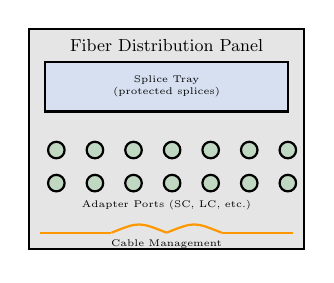
\begin{tikzpicture}[scale=0.7, every node/.style={transform shape}]
                % Fiber distribution panel
                \draw[thick, fill=gray!20] (0,0) rectangle (5,4);
                
                % Panel label
                \node[font=\small] at (2.5,3.7) {Fiber Distribution Panel};
                
                % Splice tray
                \draw[thick, fill=networkblue!20] (0.3,2.5) rectangle (4.7,3.4);
                \node[font=\tiny, text width=3cm, align=center] at (2.5,2.95) {Splice Tray\\(protected splices)};
                
                % Adapter panel ports
                \foreach \x in {0.5,1.2,1.9,2.6,3.3,4.0,4.7} {
                    \draw[thick, fill=networkgreen!30] (\x,1.8) circle (0.15);
                }
                \foreach \x in {0.5,1.2,1.9,2.6,3.3,4.0,4.7} {
                    \draw[thick, fill=networkgreen!30] (\x,1.2) circle (0.15);
                }
                \node[font=\tiny] at (2.5,0.8) {Adapter Ports (SC, LC, etc.)};
                
                % Cable management
                \draw[thick, networkorange] (0.2,0.3) -- (1.5,0.3);
                \draw[thick, networkorange] (1.5,0.3) .. controls (2,0.5) .. (2.5,0.3);
                \draw[thick, networkorange] (2.5,0.3) .. controls (3,0.5) .. (3.5,0.3);
                \draw[thick, networkorange] (3.5,0.3) -- (4.8,0.3);
                \node[font=\tiny] at (2.5,0.1) {Cable Management};
            \end{tikzpicture}
        \end{column}
    \end{columns}
\end{frame}

% Slide 33: Advanced Fiber: WDM and Multi-Fiber
\begin{frame}{Advanced Fiber Technologies}
    \begin{itemize}
        \item \textbf{Wavelength Division Multiplexing (WDM)} allows multiple signals to travel simultaneously on one fiber by using different colors (wavelengths) of light.
        \item \textbf{CWDM (Coarse WDM)} uses widely-spaced wavelengths (8-18 channels) for metro applications, while \textbf{DWDM (Dense WDM)} packs 40-80+ channels tightly for long-haul networks.
        \item \textbf{MPO/MTP connectors} are multi-fiber connectors that terminate 12 or 24 fibers in a single small connector, dramatically reducing installation time in data centers.
        \item These technologies are primarily used in telecommunications and large data centers where maximizing fiber capacity is critical.
    \end{itemize}
    
    \vspace{0.3cm}
    \begin{block}{Think of WDM Like This}
        WDM is like having multiple radio stations broadcasting simultaneously---each uses a different frequency so they don't interfere. With fiber, different colors of light act as separate "channels."
    \end{block}
\end{frame}

% Slide 34: Copper vs. Fiber Comparison
\begin{frame}{Copper vs. Fiber: Making the Choice}
    \begin{table}
        \centering
        \small
        \begin{tabular}{|l|c|c|}
            \hline
            \rowcolor{networkblue!20}
            \textbf{Feature} & \textbf{Copper (UTP)} & \textbf{Fiber Optic} \\
            \hline
            Maximum Distance & 100 m & 550 m - 40+ km \\
            \hline
            Maximum Speed & 10 Gbps (Cat 6a) & 100+ Gbps \\
            \hline
            EMI Immunity & Vulnerable & Completely immune \\
            \hline
            Installation Cost & Lower & Higher \\
            \hline
            Installation Difficulty & Easier & Requires training \\
            \hline
            Security & Can be tapped & Very difficult to tap \\
            \hline
            Weight & Heavier & Much lighter \\
            \hline
            Power Delivery & Yes (PoE) & No \\
            \hline
        \end{tabular}
    \end{table}
    
    \vspace{0.3cm}
    \begin{block}{Decision Guide}
        Use copper for: workstation connections, short runs, PoE devices. Use fiber for: building-to-building, long distances, high EMI environments, high-speed backbones.
    \end{block}
\end{frame}

% Slide 35: CASE STUDY - Problem
\begin{frame}{Case Study: The Addams Family Estate Network}
    \begin{block}{The Scenario}
        \scriptsize
        The Addams family has purchased the abandoned estate next door to expand their property. Gomez wants to connect the network in the main mansion to the new guest house, which will serve as Pugsley's laboratory for explosive experiments.
        
        \vspace{0.3cm}
        Key facts:
        \begin{itemize}
            \item Distance between buildings: 800 meters
            \item The path runs near high-voltage power lines that feed Fester's electrical experiments
            \item Current network requirement: 1 Gbps minimum
            \item Future plans: Upgrade to 10 Gbps within 3 years
            \item Budget: Moderate (this is the Addams family, after all)
        \end{itemize}
    \end{block}
    
    \vspace{0.3cm}
    \textbf{Your Task:}
    \begin{itemize}
        \item What cable type should they use and why?
        \item If choosing fiber, should they use single-mode or multimode?
    \end{itemize}
\end{frame}

% Slide 36: CASE STUDY - Solution
\begin{frame}{Case Study: Solution}
    \textbf{Correct Solution:} Single-Mode Fiber (1000BASE-LX or 10GBASE-LR)
    
    \vspace{0.3cm}
    \begin{itemize}
        \small
        \item \textbf{Copper Eliminated:} 800 meters far exceeds the 100-meter limit for copper Ethernet---copper is not an option
        \item \textbf{EMI Immunity:} High-voltage power lines would destroy copper signals; fiber is completely immune to electromagnetic interference
        \item \textbf{Distance Capability:} Single-mode fiber easily handles 800m (can go 10+ km); multimode limited to 550m maximum
        \item \textbf{Future-Proofing:} Single-mode supports both current 1 Gbps (1000BASE-LX) and future 10 Gbps (10GBASE-LR) requirements
        \item \textbf{Why Not Multimode?} At 800m, multimode won't work---it exceeds the 550m limit even for 1 Gbps
    \end{itemize}
    
    \vspace{0.3cm}
    \begin{alertblock}{Final Recommendation}
        Install single-mode fiber with 1000BASE-LX equipment now, upgrade to 10GBASE-LR transceivers later without replacing cables. The higher upfront cable cost is offset by long-term flexibility.
    \end{alertblock}
\end{frame}


% Slide 37: The Physical Environment Matters
\begin{frame}{The Physical Environment Matters}
    \begin{itemize}
        \item Network equipment needs more than just cables---servers, switches, and routers require carefully controlled physical environments to operate reliably.
        \item \textbf{Equipment rooms} and \textbf{data centers} must maintain specific temperature, humidity, and power conditions to prevent hardware failure.
        \item Environmental problems cause the majority of unexpected network downtime: overheating servers, power outages, water damage, and fire.
        \item Understanding physical infrastructure requirements is essential because even the best network design fails if equipment shuts down due to environmental issues.
    \end{itemize}
    
    \vspace{0.3cm}
    \begin{alertblock}{Real-World Impact}
        A single equipment room cooling failure can take down an entire building's network in minutes, affecting hundreds or thousands of users. Environmental monitoring is not optional.
    \end{alertblock}
\end{frame}

% Slide 38: Rack Systems
\begin{frame}{Rack Systems}
    \begin{columns}[T]
        \begin{column}{0.55\textwidth}
            \begin{itemize}
                \item \textbf{19-inch equipment racks} are the standard mounting system for network equipment, servers, and patch panels in professional installations.
                \item Rack height is measured in \textbf{U units} (rack units), where 1U equals 1.75 inches---a typical rack is 42U tall.
                \item Equipment includes mounting rails, cable management arms, vertical power strips, and proper airflow management (front-to-back or bottom-to-top).
                \item \textbf{Cable management} within racks prevents tangled "spaghetti" connections and ensures proper airflow around heat-generating equipment.
            \end{itemize}
        \end{column}
        \begin{column}{0.4\textwidth}
            \centering
            \includegraphics[width=0.95\textwidth]{network_rack_diagram.png}
            
            \vspace{0.2cm}
            \small{\textit{Standard network rack showing switches, patch panels, and cable management}}
        \end{column}
    \end{columns}
\end{frame}

% Slide 39: Temperature and Humidity Control
\begin{frame}{Temperature and Humidity Control}
    \begin{itemize}
        \item Network equipment should operate in temperatures between 68-77°F (20-25°C)---exceeding these ranges causes hardware to throttle performance or shut down completely.
        \item \textbf{Humidity} must stay between 40-60\% because low humidity causes static discharge (which damages electronics) and high humidity causes condensation (which shorts circuits).
        \item Data centers use precision \textbf{HVAC systems} specifically designed for equipment cooling, not human comfort, with redundant cooling units.
        \item \textbf{Hot aisle/cold aisle} design arranges racks so equipment air intakes face one direction (cold aisle) and exhausts face the opposite direction (hot aisle), maximizing cooling efficiency.
    \end{itemize}
    
    \vspace{0.3cm}
    \begin{block}{Warning Signs}
        If equipment rooms feel warm to touch, have high fan noise, or show temperature warnings, the cooling system is inadequate and equipment lifespan is being drastically reduced.
    \end{block}
\end{frame}

% Slide 40: Power Management
\begin{frame}{Power Management}
    \begin{itemize}
        \item An \textbf{Uninterruptible Power Supply (UPS)} provides battery backup that keeps equipment running during power outages and conditions power to prevent damage from surges and sags.
        \item UPS runtime typically ranges from 5-30 minutes---enough time for graceful shutdown or for backup generators to start.
        \item \textbf{Surge protectors} only block voltage spikes; true UPS systems also provide battery backup and clean, regulated power continuously.
        \item Critical facilities use \textbf{redundant power supplies} in servers (two power supplies, two circuits) and backup generators that automatically start within seconds of power loss.
    \end{itemize}
    
    \vspace{0.3cm}
    \begin{alertblock}{Investment Priority}
        A quality UPS protecting \$50,000 of network equipment costs \$2,000-5,000---cheap insurance against power problems that could cause equipment failure or data loss.
    \end{alertblock}
\end{frame}

% Slide 41: Fire Suppression in Equipment Rooms
\begin{frame}{Fire Suppression in Equipment Rooms}
    \begin{itemize}
        \item Traditional water sprinkler systems will destroy electronic equipment---water and electricity create short circuits that ruin servers, switches, and data.
        \item \textbf{Clean agent systems} (like FM-200) use gaseous chemicals that suppress fire without leaving residue or conducting electricity, allowing equipment to continue operating afterward.
        \item \textbf{Inert gas systems} displace oxygen in the room, suffocating the fire without using chemicals or water.
        \item \textbf{Pre-action systems} provide a warning (alarm and detection) before releasing suppressant, giving personnel time to verify it's a real fire and evacuate.
        \item These specialized systems cost significantly more than water sprinklers but are essential for protecting valuable equipment and irreplaceable data.
    \end{itemize}
\end{frame}

% Slide 42: Cable Troubleshooting Introduction
\begin{frame}{Cable Troubleshooting Introduction}
    \begin{itemize}
        \item "It was working yesterday!"---This is the most common phrase technicians hear, and now you need to figure out what changed.
        \item A \textbf{systematic approach} beats random guessing: gather information, form hypotheses, test methodically, and document your findings.
        \item Good \textbf{documentation} is your best friend during troubleshooting---cable labels, network diagrams, and installation records save hours of work.
        \item Most cable problems fall into a few common categories: physical damage, incorrect termination, exceeded specifications, or environmental interference.
    \end{itemize}
    
    \vspace{0.3cm}
    \begin{block}{The Troubleshooting Mindset}
        Start with the simple, obvious causes (loose connection, wrong cable) before assuming complex problems. The solution is usually simpler than you think.
    \end{block}
\end{frame}

% Slide 43: Common Cable Problems
\begin{frame}{Common Cable Problems}
    \begin{table}
        \centering
        \small
        \begin{tabular}{|p{3cm}|p{3.5cm}|p{3.5cm}|}
            \hline
            \rowcolor{networkblue!20}
            \textbf{Symptom} & \textbf{Possible Cause} & \textbf{Solution} \\
            \hline
            No connectivity & Unplugged cable, broken wire, bad crimp & Check connections, test cable, re-terminate \\
            \hline
            Intermittent drops & Damaged cable, loose connection, marginal crimp & Replace cable, secure connections \\
            \hline
            Slow speeds & Wrong cable category, excessive length, bad termination & Verify Cat rating, check distance, re-terminate \\
            \hline
            Short max distance & Attenuation too high, cable too long, wrong category & Test with certifier, check length, upgrade cable \\
            \hline
            Errors/corruption & Interference (EMI/RFI), crosstalk, poor grounding & Shield cable, reroute away from noise, check grounds \\
            \hline
        \end{tabular}
    \end{table}
    
    \vspace{0.2cm}
    \small{\textit{Always test methodically---don't assume the cable is bad until you've verified it with proper tools}}
\end{frame}

% Slide 44: Cable Testing Tools
\begin{frame}{Cable Testing Tools}
    \begin{itemize}
        \item A \textbf{cable certifier} tests cables against industry standards (TIA/EIA), measuring attenuation, near-end crosstalk, return loss, and providing pass/fail certification (expensive but essential for professional installations).
        \item \textbf{Wire map testers} verify that all 8 wires are connected to the correct pins and detect opens, shorts, reversed pairs, and split pairs (inexpensive, basic testing).
        \item \textbf{Tone generators and probes} send an audible signal through a cable while you use the probe to trace which physical cable it is among many (essential for identifying unlabeled cables).
        \item \textbf{Optical Time Domain Reflectometers (OTDR)} test fiber optic cables by sending light pulses and measuring reflections to locate breaks and measure loss (advanced, expensive).
    \end{itemize}
    
    \vspace{0.3cm}
    \begin{block}{Tool Investment}
        Basic wire map tester: \$50-100. Professional cable certifier: \$2,000-5,000. Choose tools based on whether you're doing occasional fixes or professional installations requiring certification.
    \end{block}
\end{frame}

% Slide 45: Understanding Cable Issues
\begin{frame}{Understanding Cable Issues}
    \begin{itemize}
        \item \textbf{Attenuation} is signal loss over distance---the signal weakens as it travels, eventually becoming too weak to detect reliably (measured in decibels, dB).
        \item \textbf{Electromagnetic Interference (EMI)} and \textbf{Radio Frequency Interference (RFI)} are external electrical noise from motors, fluorescent lights, radio transmitters, and power lines that corrupts network signals.
        \item \textbf{Near-End Crosstalk (NEXT)} occurs when signal from one wire pair bleeds into adjacent pairs near the transmission end, causing interference.
        \item \textbf{Far-End Crosstalk (FEXT)} is similar bleeding between pairs but measured at the far end of the cable.
        \item \textbf{Return loss} measures signal reflection caused by impedance mismatches---like sound echoing back when you shout into a canyon.
    \end{itemize}
    
    \vspace{0.2cm}
    \begin{block}{The Bottom Line}
        Quality cables, proper termination, correct installation, and appropriate shielding prevent most of these issues. Cheap cables and sloppy work create expensive problems.
    \end{block}
\end{frame}

% Slide 46: CASE STUDY - Problem
\begin{frame}{Case Study: The Addams Family Network Mystery}
    \begin{block}{The Scenario}
        Lurch reports that the network connection in the conservatory keeps dropping every few minutes. Other users on the same switch in the telecommunications room work perfectly. Wednesday investigates and finds:
        
        \vspace{0.3cm}
        \begin{itemize}
            \item The cable from the wall jack to Morticia's computer works fine (tested with cable tester)
            \item The patch cable in the telecom room connecting patch panel to switch also tests good
            \item The conservatory is 85 meters from the telecom room
            \item The horizontal cable was installed last year and was working fine until this week
            \item The conservatory is next to Fester's workshop, where he recently installed several large Tesla coils for experiments
        \end{itemize}
    \end{block}
    
    \vspace{0.3cm}
    \textbf{Your Task:} What should Wednesday check next? What is the most likely cause? How would you troubleshoot this systematically?
\end{frame}

% Slide 47: CASE STUDY - Solution
\begin{frame}{Case Study: Solution}
    \textbf{Most Likely Cause:} Electromagnetic interference from Fester's Tesla coils
    
    \vspace{0.3cm}
    \textbf{Troubleshooting Steps:}
    \begin{enumerate}
        \item Use a cable certifier (not just a basic tester) to check the horizontal cable run for interference and crosstalk---basic testers won't detect EMI issues
        \item Test the connection when Fester's Tesla coils are powered off---if it works, you've confirmed the interference source
        \item Check if the cable runs parallel to power lines or near Fester's equipment
        \item Measure actual error rates and packet loss (not just "it drops sometimes")
    \end{enumerate}
    
    \vspace{0.3cm}
    \textbf{Solutions (in order of preference):}
    \begin{itemize}
        \item Reroute the cable away from Fester's workshop (maintain 12+ inches from interference sources)
        \item Replace with shielded twisted pair (STP) cable properly grounded
        \item Use fiber optic cable (completely immune to EMI, but most expensive)
    \end{itemize}
\end{frame}

% Slide 48: Conclusion - Bringing It All Together
\begin{frame}{Conclusion: The Foundation of Every Network}
    \textbf{Key Takeaways:}
    \begin{itemize}
        \item The physical layer is the foundation---every network depends on properly installed, maintained cabling infrastructure.
        \item Choose the right cable for each situation: consider distance, speed requirements, environment, interference, and future needs.
        \item Standards exist for good reasons: they ensure safety, compatibility, performance, and long-term reliability.
        \item Proper installation prevents 90\% of problems: correct termination, appropriate cable ratings, good documentation, and following specifications.
        \item Systematic troubleshooting beats random guessing: use the right tools, test methodically, and document everything.
    \end{itemize}
    
    \vspace{0.3cm}
    \begin{block}{Your Impact}
        As a network technician, your cabling work keeps businesses running, students learning, hospitals operating, and families connected. Quality work at the physical layer makes everything else possible.
    \end{block}
    
    \vspace{0.2cm}
    \textbf{Next Steps:} Apply these concepts in hands-on labs, pursue certifications (CompTIA Network+, BICSI RCDD), and keep learning!
\end{frame}

\end{document}